\documentclass{report}
\usepackage[utf8]{inputenc}
% \usepackage[landscape]{geometry}
\usepackage{graphicx}
\title{IVR Assignment}
\author{Maksymilian Mozolewski \& Martin Lewis}
\date{November 2020}
\newcommand\scalemath[2]{\scalebox{#1}{\mbox{\ensuremath{\displaystyle #2}}}}
\usepackage{amsmath}
\usepackage[landscape,margin=0.5in]{geometry}

\let\cos\relax
\let\sin\relax
% \DeclareMathOperator{\cos}{\mathit{C}}
% \DeclareMathOperator{\sin}{\mathit{S}}
\newcommand{\sin}[1]{\mathit{S}_{#1}}
\newcommand{\cos}[1]{\mathit{C}_{#1}}

\begin{document}

\maketitle

\section*{2.1}

The first part of this section was straight forward calculating the position of the angles based of the sinusoidal positions. This achieved with rospy's get time function and sin.

The second part was the more difficult part. I tried a few different methods, optimisation, projections but finally settling for using trigonometry. Using atan2 to find the values of
joint 2 and 3. Joint 2 is found with atan on the y and z components of the vector between the blue and green blobs. Then the vector is rotated by the found angle
and then atan is run on the x and z components for joint3. This does however mean that the uncertainly and error in the angle of joint 2 is passed to joint3.

You can see the two example sections of an rqt\_plot graph from joints 2 and 3 in figures 1 and 2.

\begin{figure}
    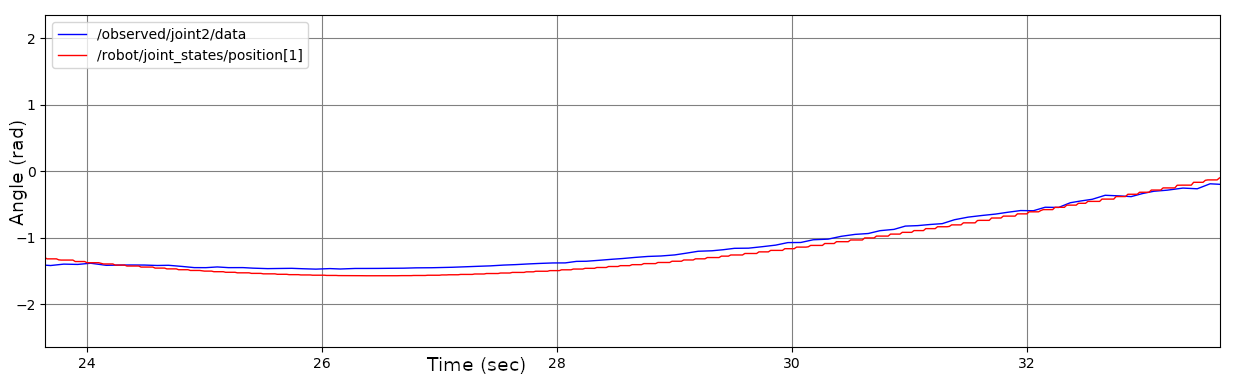
\includegraphics[width=\linewidth]{joint2.png}
    \caption{Joint2 Angle}
\end{figure}

\begin{figure}
    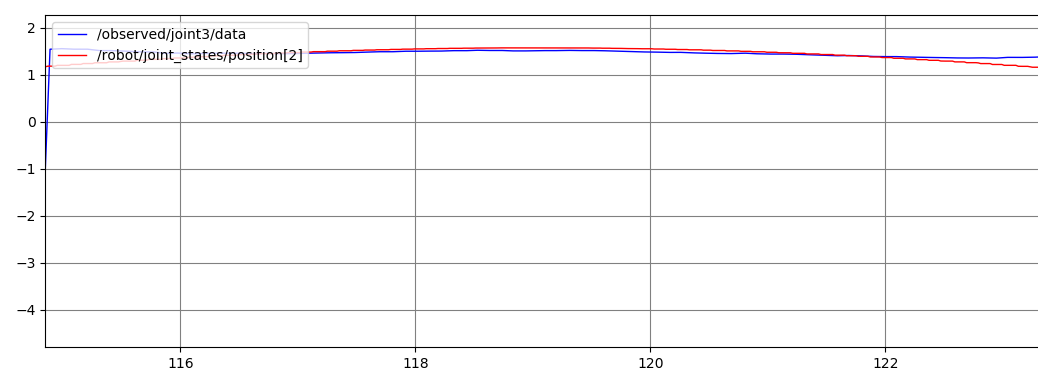
\includegraphics[width=\linewidth]{joint3.png}
    \caption{Joint3 Angle}
\end{figure}

Joint 4 however is calculated by a projection. This means its not reliant on the first two angles. It works out the angle between the vector between the
green and red blobs and the vector between the blue and green ones.

\begin{figure}
    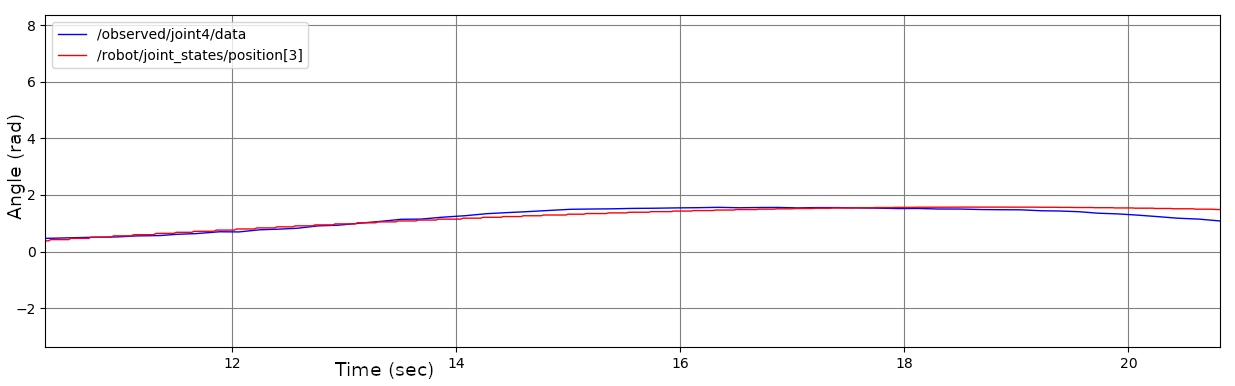
\includegraphics[width=\linewidth]{joint4.png}
    \caption{Joint4 Angle}
\end{figure}

\section*{2.2}

\section*{3.1}

The forward kinematics, was derived using d-h parameters and a sympy script which parsed it to avoid any mathematical errors (The said script is available in the repository). The final forward kinematics translation component looks like the following:

\begin{equation*}
\begin{bmatrix}
           x_{e} \\
           y_{e} \\
           z_{e}
\end{bmatrix} = 
\left(\begin{array}{c} %
    3 \left(\sin{q_{1}} \sin{q_{2}} \cos{q_{3}} + \sin{q_{3}} \cos{q_{1}}\right) \cos{q_{4}}  %
    + 3.5 \sin{q_{1}} \sin{q_{2}} \cos{q_{3}} %
    + 3 \sin{q_{1}} \sin{q_{4}} \cos{q_{2} } %
    + 3.5 \sin{q_{3}} \cos{q_{1}} %
    \\
    3 \left(\sin{q_{1}} \sin{q_{3}} %
    - \sin{q_{2}} \cos{q_{1}} \cos{q_{3}}\right) \cos{q_{4}} %
    + 3.5 \sin{q_{1}} \sin{q_{3}} %
    - 3.5 \sin{q_{2}} \cos{q_{1}} \cos{q_{3}} %
    - 3 \sin{q_{4}} \cos{q_{1}} \cos{q_{2}} %
    \\
    - 3 \sin{q_{2}} \sin{q_{4}} %
    + 3 \cos{q_{2}} \cos{q_{3}} \cos{q_{4}} %
    + 3.5 \cos{q_{2}} \cos{q_{3}} + 2.5
    \end{array}\right)
\end{equation*}


\begin{equation*}
\begin{bmatrix}
           \dot{x_{e}} \\
           \dot{y_{e}} \\
           \dpt{z_{e}}
\end{bmatrix} = %
\left(\begin{array}{c}\dot{q_{1}} \left(\left(- 3 \sin{\left(q_{1} \right)} \sin{\left(q_{3} \right)} + 3 \sin{\left(q_{2} \right)} \cos{\left(q_{1} \right)} \cos{\left(q_{3} \right)}\right) \cos{\left(q_{4} \right)} - 3.5 \sin{\left(q_{1} \right)} \sin{\left(q_{3} \right)} + 3.5 \sin{\left(q_{2} \right)} \cos{\left(q_{1} \right)} \cos{\left(q_{3} \right)} + 3 \sin{\left(q_{4} \right)} \cos{\left(q_{1} \right)} \cos{\left(q_{2} \right)}\right) + \dot{q_{2}} \left(- 3 \sin{\left(q_{1} \right)} \sin{\left(q_{2} \right)} \sin{\left(q_{4} \right)} + 3 \sin{\left(q_{1} \right)} \cos{\left(q_{2} \right)} \cos{\left(q_{3} \right)} \cos{\left(q_{4} \right)} + 3.5 \sin{\left(q_{1} \right)} \cos{\left(q_{2} \right)} \cos{\left(q_{3} \right)}\right) + \dot{q_{3}} \left(\left(- 3 \sin{\left(q_{1} \right)} \sin{\left(q_{2} \right)} \sin{\left(q_{3} \right)} + 3 \cos{\left(q_{1} \right)} \cos{\left(q_{3} \right)}\right) \cos{\left(q_{4} \right)} - 3.5 \sin{\left(q_{1} \right)} \sin{\left(q_{2} \right)} \sin{\left(q_{3} \right)} + 3.5 \cos{\left(q_{1} \right)} \cos{\left(q_{3} \right)}\right) + \dot{q_{4}} \left(- \left(3 \sin{\left(q_{1} \right)} \sin{\left(q_{2} \right)} \cos{\left(q_{3} \right)} + 3 \sin{\left(q_{3} \right)} \cos{\left(q_{1} \right)}\right) \sin{\left(q_{4} \right)} + 3 \sin{\left(q_{1} \right)} \cos{\left(q_{2} \right)} \cos{\left(q_{4} \right)}\right)\\\dot{q_{1}} \left(\left(3 \sin{\left(q_{1} \right)} \sin{\left(q_{2} \right)} \cos{\left(q_{3} \right)} + 3 \sin{\left(q_{3} \right)} \cos{\left(q_{1} \right)}\right) \cos{\left(q_{4} \right)} + 3.5 \sin{\left(q_{1} \right)} \sin{\left(q_{2} \right)} \cos{\left(q_{3} \right)} + 3 \sin{\left(q_{1} \right)} \sin{\left(q_{4} \right)} \cos{\left(q_{2} \right)} + 3.5 \sin{\left(q_{3} \right)} \cos{\left(q_{1} \right)}\right) + \dot{q_{2}} \left(3 \sin{\left(q_{2} \right)} \sin{\left(q_{4} \right)} \cos{\left(q_{1} \right)} - 3 \cos{\left(q_{1} \right)} \cos{\left(q_{2} \right)} \cos{\left(q_{3} \right)} \cos{\left(q_{4} \right)} - 3.5 \cos{\left(q_{1} \right)} \cos{\left(q_{2} \right)} \cos{\left(q_{3} \right)}\right) + \dot{q_{3}} \left(\left(3 \sin{\left(q_{1} \right)} \cos{\left(q_{3} \right)} + 3 \sin{\left(q_{2} \right)} \sin{\left(q_{3} \right)} \cos{\left(q_{1} \right)}\right) \cos{\left(q_{4} \right)} + 3.5 \sin{\left(q_{1} \right)} \cos{\left(q_{3} \right)} + 3.5 \sin{\left(q_{2} \right)} \sin{\left(q_{3} \right)} \cos{\left(q_{1} \right)}\right) + \dot{q_{4}} \left(- \left(3 \sin{\left(q_{1} \right)} \sin{\left(q_{3} \right)} - 3 \sin{\left(q_{2} \right)} \cos{\left(q_{1} \right)} \cos{\left(q_{3} \right)}\right) \sin{\left(q_{4} \right)} - 3 \cos{\left(q_{1} \right)} \cos{\left(q_{2} \right)} \cos{\left(q_{4} \right)}\right)\\\dot{q_{2}} \left(- 3 \sin{\left(q_{2} \right)} \cos{\left(q_{3} \right)} \cos{\left(q_{4} \right)} - 3.5 \sin{\left(q_{2} \right)} \cos{\left(q_{3} \right)} - 3 \sin{\left(q_{4} \right)} \cos{\left(q_{2} \right)}\right) + \dot{q_{3}} \left(- 3 \sin{\left(q_{3} \right)} \cos{\left(q_{2} \right)} \cos{\left(q_{4} \right)} - 3.5 \sin{\left(q_{3} \right)} \cos{\left(q_{2} \right)}\right) + \dot{q_{4}} \left(- 3 \sin{\left(q_{2} \right)} \cos{\left(q_{4} \right)} - 3 \sin{\left(q_{4} \right)} \cos{\left(q_{2} \right)} \cos{\left(q_{3} \right)}\right)\end{array}\right)
\end{equation*}

\end{document}
